%!TEX root = ../main.tex
\vspace{-0.5em}
\subsection{Sensitivity Analysis}
\label{exp:sec:sensitivity}

\begin{figure}[t]   
	\centering
	\begin{minipage}[t]{0.38\textwidth}
		\centering
		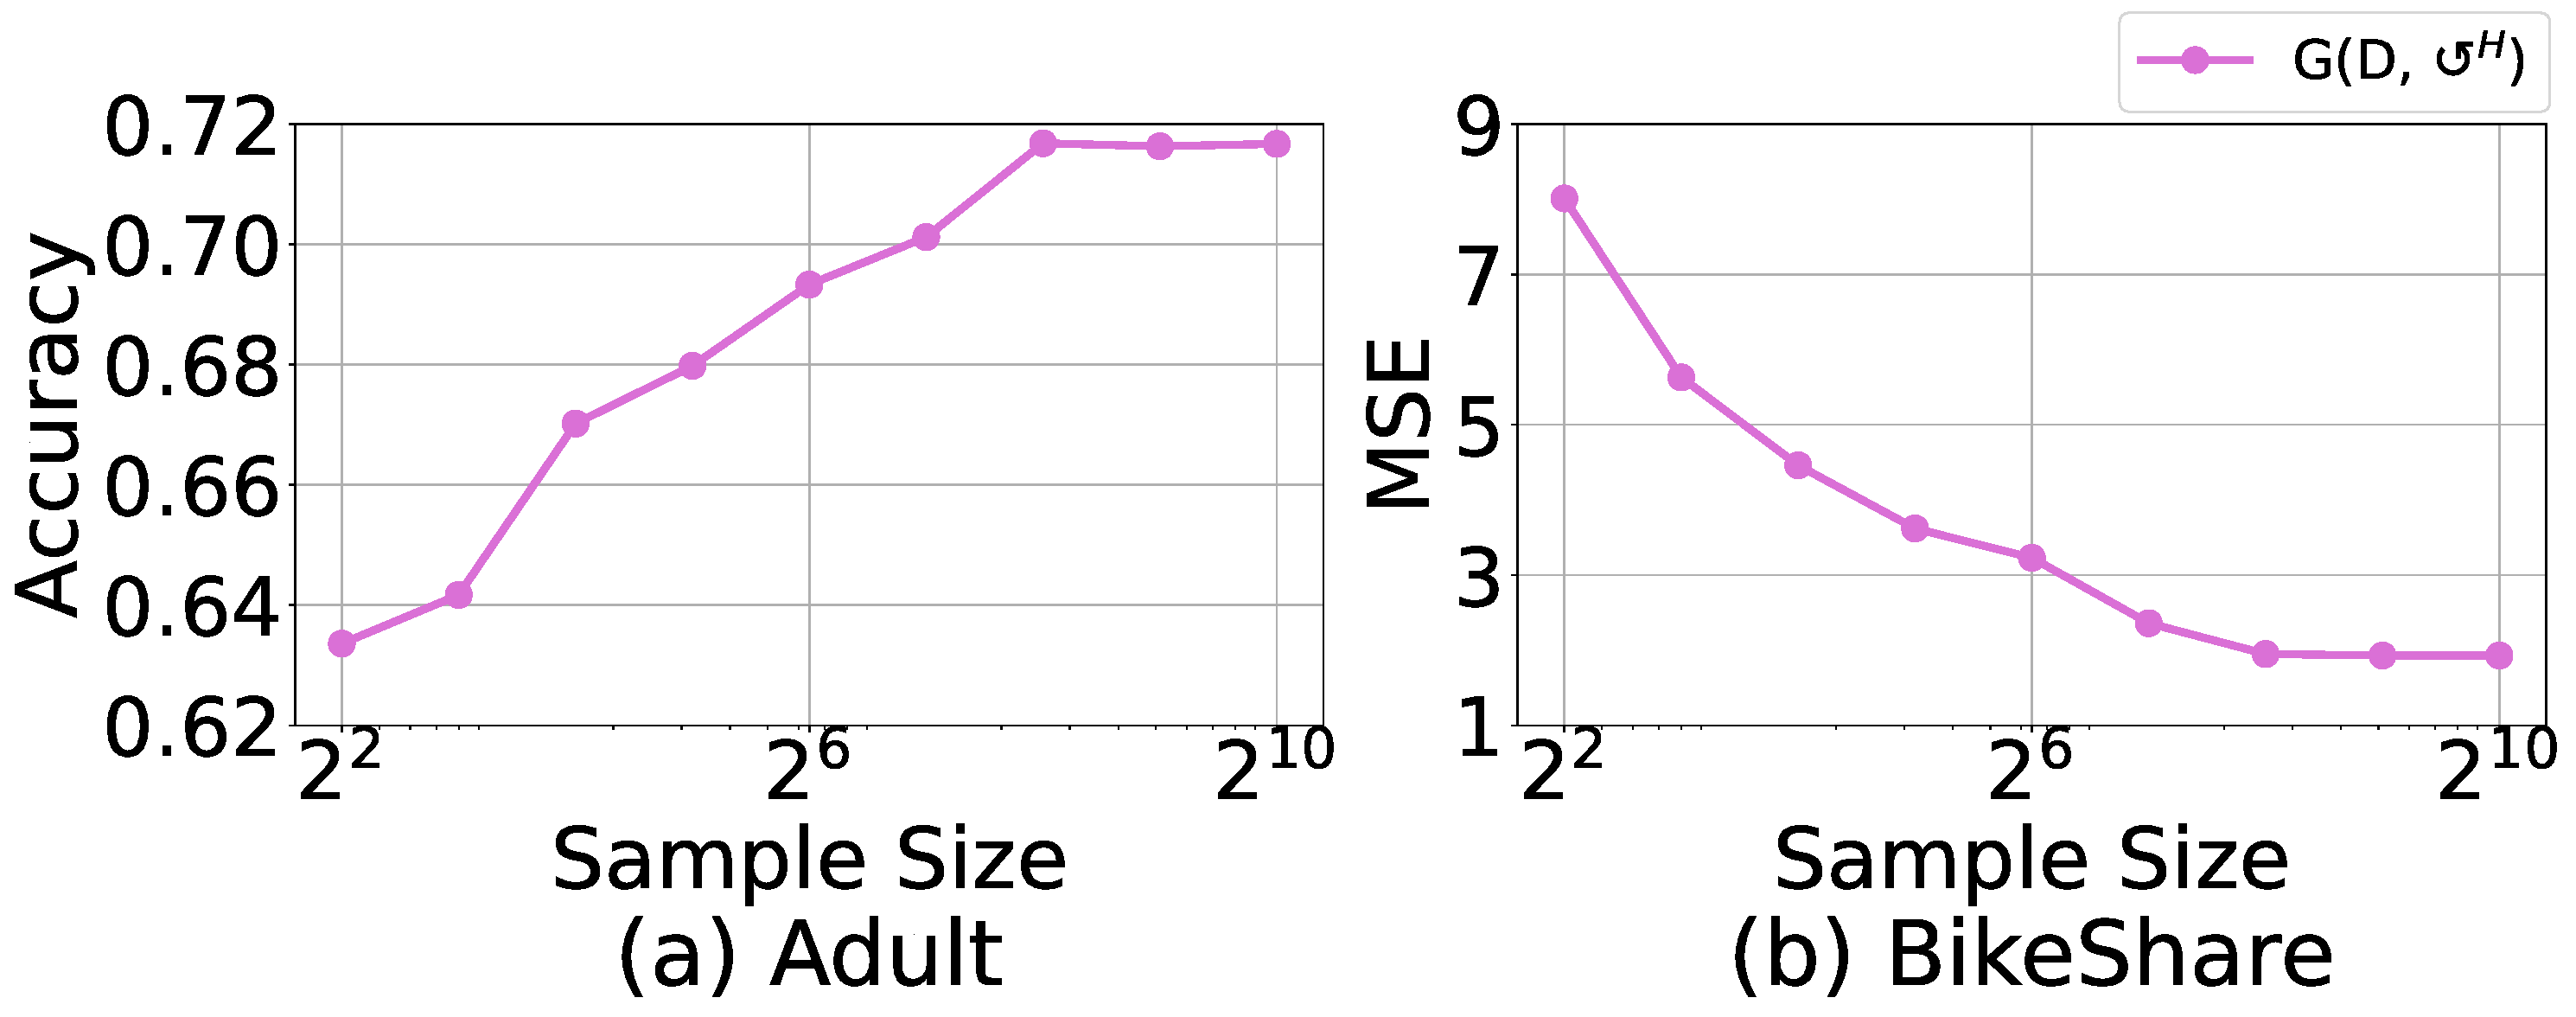
\includegraphics[width=\columnwidth]{figs/samplesize}
		\vspace{-2.5em}
		\caption{Varying sample size.}
		\label{fig:samplesize}
	\end{minipage}
	\begin{minipage}[t]{0.58\textwidth}
		\centering
		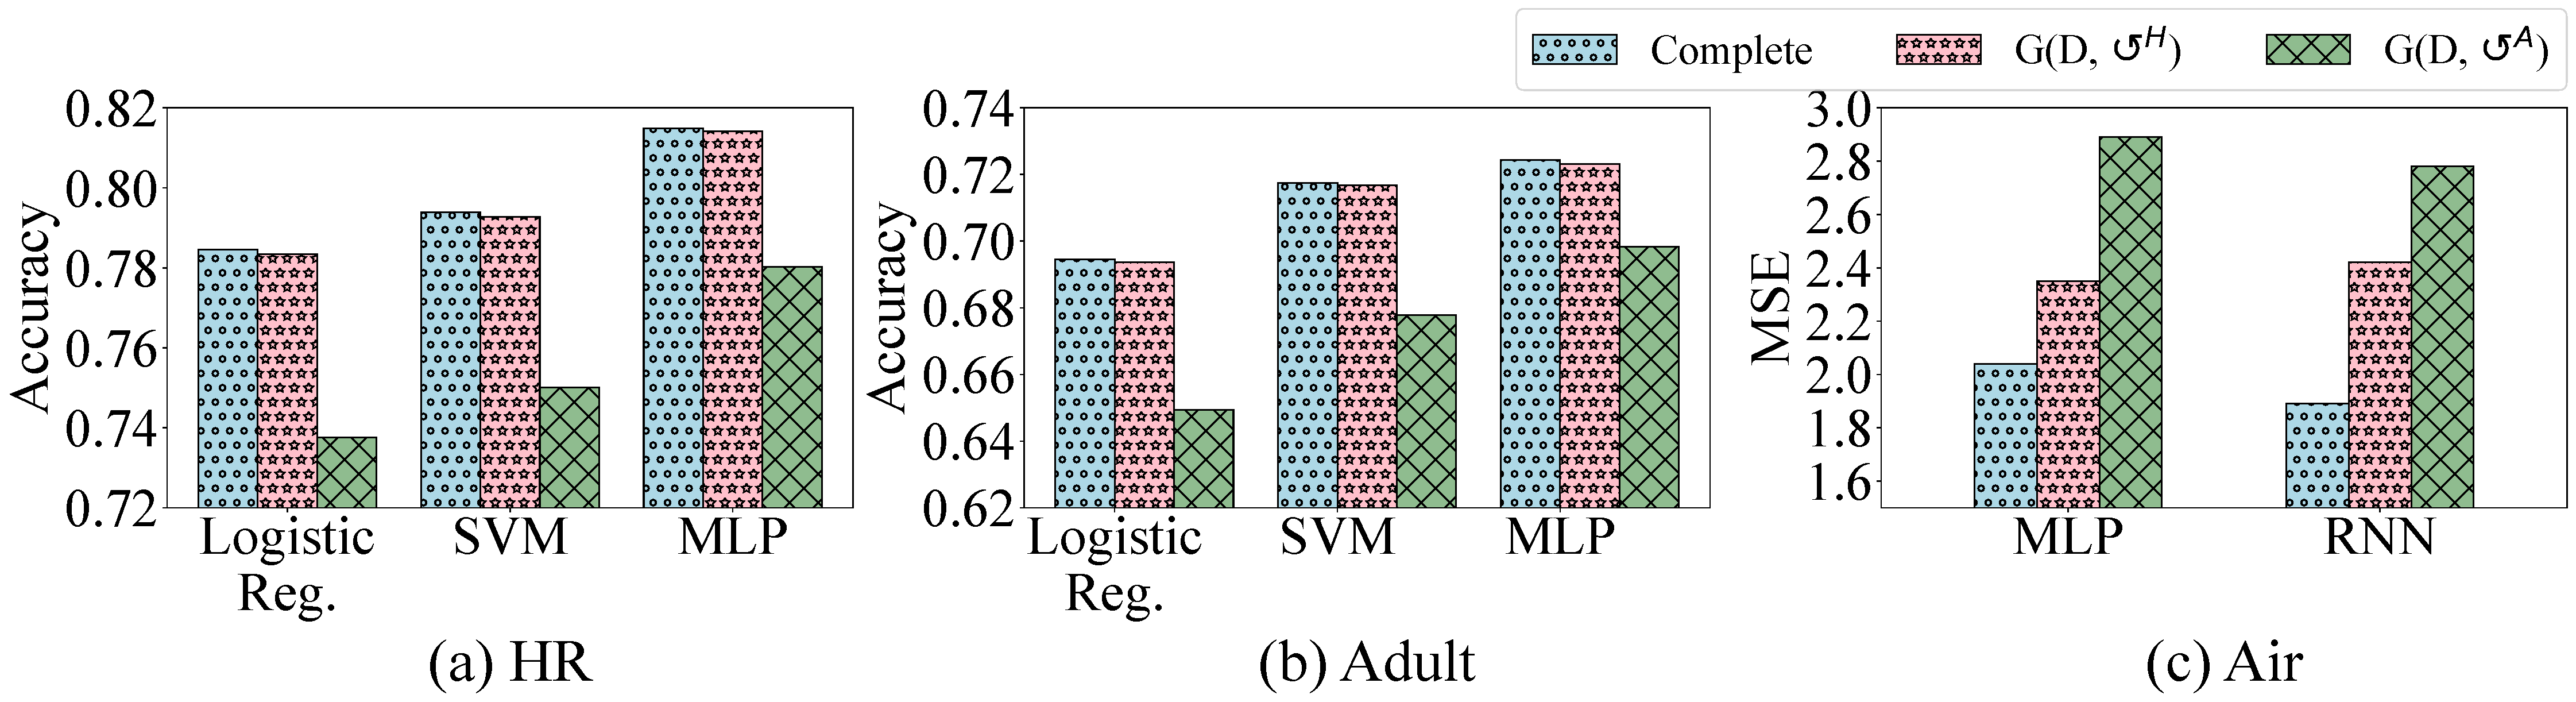
\includegraphics[width=\columnwidth]{figs/downstream_all}
		\vspace{-2.5em}
		\caption{Varying downstream model.}
		\label{fig:downmodel}
	\end{minipage}
	\vspace*{-1em}   
\end{figure}


\noindent{\bf Varying the sample size.} In this part, we vary the sample size $h$ and evaluate the performance. The experimental results are shown in Figure~\ref{fig:samplesize}. We vary the sample size $h$ from $2^2$ to $2^{10}$. We can see that when $h$ is too small, the performance is low. The reason is that \ours cannot precisely estimate the utilities of tuples when $h$ is  small.  When the sample size increases, we can see that the performance improves rapidly and finally becomes stable, which indicates that \ours is not much sensitive to the sample size when $h$ is not too small.

\noindent{\bf Varying the downstream models.} Recap that \ours can be used on different convex models. Thus, in this part, we apply \ours on different convex models and evaluate the performance. We evaluate logistic regression and SVM for classification tasks. For regression tasks, we evaluate linear regression, ridge regression and SVM regression. We can see that  in Figure~\ref{fig:downmodel} (a) and (b), on dataset \adult, $\seven$ achieved 71.7\% accuracy for SVM, better than on logistic regression (69.4\%). Although different downstream models may have different performance, \ours can improve the model performance for the specific downstream model. In order to show that \ours can be used for other types of models like neural networks, we compare with Multilayer Perceptron (MLP, fully connected networks of 2 hidden layers with 256 nodes for each layer), although \ours does not hold
theoretical guarantee for this non-convex model. As shown in Figure~\ref{fig:downmodel}, we can see that MLP achieves almost the same performance as the ground truth. This is because the coreset selected by \ours can also represent the full dataset. However, in Figure~\ref{fig:downmodel}(c), on a large dataset \air (with metric MSE, the lower the better), neural network based methods (we also implement RNN, 2 hidden layers with 128 nodes for each layer) can have a better accuracy but the coreset cannot perfectly achieve the same performance. %Since we need to compare $\seven$ and $\eight$ with $\truth$, we drop the incomplete tuples in the original dataset and manually inject missing values. 
This may because this large dataset has more informative things to learn, and it is hard for the coreset-based solution to well represent the dataset without the theoretical guarantee.


%\add{For the MLP model, we use fully connected networks of 2 hidden layers. Each layer has 256 nodes. We find that \ours failed on \air when using non-convex model. In Figure~\ref{fig:downmodel}, we can see that MLP (2 hidden layers with 256 nodes for each layer) and RNN (2 hidden layers with 128 nodes for each layer) trained on coreset cannot achieve the same performance on the full dataset.}

%\cc{details of MLP and RNN}

\noindent{\bf Varying the percentage of incomplete tuples.} In this part, we vary the rate of missing tuples and evaluate the performance, as shown in Figure~\ref{fig:vary_misstuple_all}. 
Note that the rate  denotes the percentage of incomplete tuples rather than the cell values. Even if a tuple just has one missing attribute, it is regarded as incomplete.	
	We vary the percentage  from $20\%$ to $100\%$. We can observe that the performance does not decrease  much with the percentage increasing from $20\%$ to $50\%$, which indicates that \ours is not very sensitive to the percentage of incomplete tuples in this range. After that, the accuracy decreases because there are more missing tuples.

Besides, we also vary the rate of missing cell values in Figure~\ref{fig:realmissrate}. In this scenario, for example, 50\% missing values of a dataset  indicates more number of missing cell values than the scenario of 50\% missing tuples. Hence, we can see that the accuracy decreases more quickly than Figure~\ref{fig:vary_misstuple_all}.



